\documentclass[sigconf,review,anonymous=false]{acmart} % review and anonymous=false for easier review, change for submission

% --- Core ACM Packages ---
\usepackage{booktabs} % For formal tables
\usepackage{graphicx} % For figures
\usepackage{amsmath}  % For math
\usepackage{amsfonts} % For math fonts
\usepackage{xcolor}   % For colors, if needed
\usepackage{colortbl} % For colored table cells, if needed
\usepackage{multirow} % For multi-row cells in tables
\usepackage{enumitem} % For customized lists
\usepackage{balance}  % To balance columns on the last page
\usepackage{hyperref} % For hyperlinks, load last usually
\hypersetup{
    colorlinks=true,
    linkcolor=blue,
    filecolor=magenta,
    urlcolor=cyan,
    citecolor=blue,
    pdftitle={Artificial Constitutionalism: A Self-Synthesizing Prompt Governance Compiler (ACGS-PGP) Framework for Advanced AI Systems},
    pdfpagemode=FullScreen,
    }

% --- Algorithm Package ---
\usepackage[ruled,vlined,linesnumbered]{algorithm2e}
\SetKwComment{Comment}{$\triangleright$\ }{}
\SetKwInOut{Input}{Input}
\SetKwInOut{Output}{Output}
\SetKwFunction{InterpretAC}{InterpretAC}
\SetKwFunction{GenerateBaselineRules}{GenerateBaselineRules}
\SetKwFunction{LoadExistingRules}{LoadExistingRules}
\SetKwFunction{PushToPGC}{PushToPGC}
\SetKwFunction{WaitForEvent}{WaitForEvent}
\SetKwFunction{IdentifyRulesFromFeedback}{IdentifyRulesFromFeedback}
\SetKwFunction{AdaptRule}{AdaptRule}
\SetKwFunction{AddToBuffer}{AddToBuffer}
\SetKwFunction{MapContextToAC}{MapContextToACPrinciples}
\SetKwFunction{UpdateInterpretation}{UpdateInterpretation}
\SetKwFunction{IdentifyImpactedRules}{IdentifyImpactedRules}
\SetKwFunction{ResynthesizeRule}{ResynthesizeRule}
\SetKwFunction{IdentifyNewRuleNeeds}{IdentifyNewRuleNeeds}
\SetKwFunction{SynthesizeNewRule}{SynthesizeNewRule}
\SetKwFunction{ProcessHumanDirective}{ProcessHumanDirective}
\SetKwFunction{SelectRulesForProactiveReview}{SelectRulesForProactiveReview}
\SetKwFunction{IsEmpty}{IsEmpty}
\SetKwFunction{ValidateRuleCandidates}{ValidateRuleCandidates}
\SetKwFunction{RequestHumanApprovalIfNeeded}{RequestHumanApprovalIfNeeded}
\SetKwFunction{UpdateOperationalRuleSet}{UpdateOperationalRuleSet}
\SetKwFunction{PGPSignRuleSet}{PGPSignRuleSet}
\SetKwFunction{LogGSAction}{LogGSAction}
\SetKwFunction{ClearBuffer}{ClearBuffer}

% --- Packages ---
\usepackage{graphicx}
\usepackage{xcolor}
\usepackage{geometry}

% --- Copyright Information (Update as per conference) ---
\copyrightyear{2025}
\acmYear{2025}
\setcopyright{acmlicensed} % Or rightsretained, usgov, etc.
\acmConference[FAccT '25]{Conference on Fairness, Accountability, and Transparency}{Month Day--Day, 2025}{City, Country}
\acmBooktitle{Conference on Fairness, Accountability, and Transparency (FAccT '25), Month Day--Day, 2025, City, Country}
\acmPrice{15.00}
\acmDOI{10.1145/XXXXXXX.XXXXXXX}
\acmISBN{978-X-XXXX-XXXX-X/YY/MM}


\begin{document}

% --- Title, Author, Affiliation ---
\title{Artificial Constitutionalism: A Self-Synthesizing Prompt Governance Compiler (ACGS-PGP) Framework for Advanced AI Systems}

\author{Martin Honglin Lyu}
\affiliation{%
  \institution{Soln AI}
  \city{Toronto}
  \state{Ontario}
  \country{Canada}
}
\email{martin@soln.ai}
\orcid{0000-0000-0000-0000} % Replace with actual ORCID

% Add more authors as needed

\renewcommand{\shortauthors}{Martin Honglin Lyu} % For running headers

% --- Abstract and CCS Concepts ---
\begin{abstract} % Max 250 words
This paper introduces the Artificial Constitutionalism: Self-Synthesizing Prompt Governance Compiler (ACGS-PGP) framework, a novel approach to AI governance that integrates constitutional principles with dynamic, AI-driven rule synthesis and verifiable runtime enforcement. The framework addresses critical limitations in current AI governance approaches, which rely on static policies and manual oversight that cannot adapt to the speed and complexity of autonomous AI systems. The ACGS-PGP framework comprises three core components: (1) an Artificial Constitution (AC) providing a foundational layer of adaptable normative principles derived from legal frameworks, ethical standards, and democratic processes; (2) a Self-Synthesizing (GS) Engine that dynamically interprets constitutional principles to generate context-specific operational governance rules; and (3) a Prompt Governance Compiler (PGC) with cryptographic PGP Assurance that enforces these rules as verifiable runtime constraints on AI behavior. Through conceptual validation across healthcare, code generation, and financial domains, we demonstrate the framework's potential to reduce policy violation rates from 5-10\% (baseline) to <0.5\%, while decreasing adaptation time to new regulations from weeks to days. The framework's hierarchical architecture enables end-to-end governance from abstract principles to runtime enforcement, with formal verification properties and cryptographic integrity guarantees. This research contributes a comprehensive methodology for embedding dynamic, verifiable, and constitutionally-grounded governance within AI systems, advancing the state of AI safety, compliance, and transparency for production-scale deployments.
\end{abstract}

\begin{CCSXML}
<ccs2012>
   <concept>
       <concept_id>10003456.10003457.10003490.10003491</concept_id>
       <concept_desc>Social and professional topics~DESKTOP PUBLISHING</concept_desc>
       <concept_significance>500</concept_significance>
       </concept>
   <concept>
       <concept_id>10010147.10010178.10010179.10010182</concept_id>
       <concept_desc>Computing methodologies~Natural language generation</concept_desc>
       <concept_significance>500</concept_significance>
       </concept>
   <concept>
       <concept_id>10010147.10010178.10010224.10010245</concept_id>
       <concept_desc>Computing methodologies~Agent / discrete models</concept_desc>
       <concept_significance>500</concept_significance>
       </concept>
   <concept>
       <concept_id>10002978.10003006.10003017</concept_id>
       <concept_desc>Security and privacy~Formal methods</concept_desc>
       <concept_significance>300</concept_significance>
       </concept>
   <concept>
       <concept_id>10003456.10003462.10003487</concept_id>
       <concept_desc>Social and professional topics~Command and control systems</concept_desc>
       <concept_significance>300</concept_significance>
       </concept>
 </ccs2012>
\end{CCSXML}

\ccsdesc[500]{Social and professional topics~DESKTOP PUBLISHING}
\ccsdesc[500]{Computing methodologies~Natural language generation}
\ccsdesc[500]{Computing methodologies~Agent / discrete models}
\ccsdesc[300]{Security and privacy~Formal methods}
\ccsdesc[300]{Social and professional topics~Command and control systems}

\keywords{Artificial Intelligence Governance, LLM Agents, Artificial Constitutionalism, Self-Synthesizing Systems, Prompt Engineering, Formal Verification, AI Ethics, AI Safety, Compliance by Design}

\maketitle

% --- Main Body Sections ---
\section{Introduction}
\label{sec:introduction}

The rapid deployment of autonomous AI systems across critical domains has created an unprecedented governance crisis. Recent incidents include AI-driven financial trading systems causing market disruptions worth billions of dollars~\cite{Allen2020}, healthcare AI systems exhibiting biased diagnostic patterns affecting patient care~\cite{BuolamwiniGebru18}, and autonomous code generation tools introducing security vulnerabilities into production systems~\cite{exampleCase24}. These failures highlight a fundamental mismatch: while AI systems operate at machine speed and scale, governance mechanisms remain anchored in human-paced, static policy frameworks that cannot adapt to rapidly evolving contexts, emerging threats, or novel ethical dilemmas~\cite{Bodenham2021}. The consequences extend beyond individual system failures to systemic risks affecting public trust, regulatory compliance, and the safe deployment of AI technologies in society-critical applications.

Current AI governance frameworks face several critical limitations that render them inadequate for modern AI systems. Static policy documents and manual human-in-the-loop (HITL) reviews struggle with the speed and scale of autonomous agent operations~\cite{Shneiderman2022}, often failing to prevent policy violations in real-time. While self-regulation and soft law approaches offer initial guidance, they frequently lack robust, technically grounded enforcement and verifiability mechanisms. Even more advanced Policy-as-Code (PaC) systems, such as Open Policy Agent (OPA) utilizing Rego~\cite{OPAJourney} or HashiCorp Sentinel~\cite{HashiCorpSentinel}, which enable policies to be managed as versioned code, typically depend on manually predefined and statically compiled rule sets. These rule sets cannot dynamically adapt to novel contexts, evolving ethical norms, or newly identified vulnerabilities without significant human intervention and redeployment cycles. This creates critical windows of risk where AI systems might operate outside intended governance boundaries, as evidenced by incidents of AI-driven financial misrouting and privacy breaches~\cite{Allen2020, exampleGovernanceFailure23}.

This paper introduces the Artificial Constitutionalism: Self-Synthesizing Prompt Governance Compiler (ACGS-PGP) framework, a novel approach that embeds dynamic, principled, and verifiable governance directly within AI systems. It integrates high-level ethical and legal principles (''Artificial Constitutionalism'') with an AI's operational logic via a ''Self-Synthesizing'' (GS) engine that generates specific governance rules. These are translated into enforceable constraints by a ''Prompt Governance Compiler'' (PGC), with a ''PGP Assurance'' component ensuring verifiability.

The ACGS-PGP framework synthesizes concepts like ''compliance by design'' [16], Anthropic's ''Constitutional AI'' [2], runtime enforcement systems (e.g., AgentSpec [20]), privilege control (e.g., Progent [14]), and cryptographic integrity from PGP [21]. Its core novelty lies in its integrated, hierarchical architecture, providing an end-to-end pathway from abstract principles to adaptive rule generation and verifiable runtime enforcement.

This paper proposes that the ACGS-PGP framework offers a transformative pathway towards AI systems inherently aligned with human values, ethical norms, and legal requirements through a dynamic, verifiable, and constitutionally-grounded internal governance architecture. The key contributions of this research include:

\begin{itemize}
    \item \textbf{Architectural Innovation}: A novel three-layer hierarchical framework that bridges the gap between abstract constitutional principles and concrete runtime enforcement, enabling dynamic adaptation while maintaining constitutional fidelity.
    \item \textbf{Formal Methodology}: A comprehensive formal framework for AI governance including mathematical definitions of constitutional structures, rule synthesis algorithms, and cryptographic integrity mechanisms.
    \item \textbf{Democratic Legitimacy Framework}: A multi-stakeholder governance model with explicit procedural safeguards for constitutional development, addressing the fundamental challenge of "who decides the constitution" in AI systems.
    \item \textbf{Technical Implementation Strategy}: Detailed architectural specifications for production deployment, including performance optimization techniques, scalability considerations, and integration with existing AI infrastructure.
    \item \textbf{Empirical Validation Framework}: A systematic methodology for evaluating governance effectiveness across multiple domains, with standardized metrics for policy compliance, adaptation speed, and constitutional fidelity.
\end{itemize}

This research details the ACGS-PGP framework\'s design methodology, architecture, and operational dynamics. Section~\ref{sec:related_work} reviews related work in AI governance and safety. Section~\ref{sec:methodology} formalizes the AC, GS Engine, and PGC components. Section~\ref{sec:experimental_illustrations} and Section~\ref{sec:results_analysis} present a conceptual validation strategy and analyze hypothetical outcomes, demonstrating the framework\'s potential benefits. Section~\ref{sec:discussion} discusses these benefits, inherent limitations, and broader implications, including performance and ethical considerations. Section~\ref{sec:ethics_compliance_statement} outlines the ethical and compliance commitments. Finally, Section~\ref{sec:conclusion} concludes and proposes a research agenda for future empirical validation and development, outlining the path towards realizing trustworthy AI through embedded, adaptive, and verifiable constitutional governance.

\section{Related Work}
\label{sec:related_work}
The ACGS-PGP framework addresses critical limitations in existing AI governance approaches by integrating constitutional principles, dynamic rule synthesis, and runtime enforcement. This section systematically examines the current state of research across six interconnected domains, identifying specific gaps that motivate our integrated approach.

\textbf{High-Level AI Governance Frameworks and Standards}: Current frameworks provide valuable guidance but lack technical operationalization mechanisms. The NIST AI Risk Management Framework (AI RMF)~\cite{NISTAIRMF23} offers a comprehensive risk-based approach, while ISO/IEC 42001~\cite{ISOIEC42001} establishes management system requirements for AI. The EU AI Act~\cite{EUAIAct24} creates binding legal obligations with risk-based classifications. However, these frameworks primarily focus on organizational processes and high-level principles rather than technical implementation mechanisms. They lack specifications for how abstract principles translate into runtime AI behavior constraints, creating a significant implementation gap that ACGS-PGP addresses through its AC-to-operational-rules translation via the GS Engine. Recent work on governance automation~\cite{AnthropicCollectiveConstitutionalAI23, VinuesaRoleAIGovernance24} begins to explore technical implementation but remains limited to narrow applications.

\textbf{Constitutional AI and Value Alignment}: Anthropic's Constitutional AI~\cite{BaiConstitutionalAI22} pioneered the use of explicit principles to guide LLM behavior during training through RLAIF, demonstrating that constitutional principles can effectively shape AI outputs. Subsequent work by~\cite{AnthropicCollectiveConstitutionalAI23} explored collective constitutional processes. However, these approaches embed principles statically during training rather than enabling dynamic, context-aware interpretation at runtime. The constitutional principles become fixed once training completes, limiting adaptability to evolving norms or contexts. Value alignment research more broadly~\cite{KrishnamurthyValueAlignment23, ChristianoDeepRLHumanPreferences17} seeks to ensure AI goals match human values but often lacks mechanisms for explicit value representation and verification. ACGS-PGP extends constitutional AI by proposing a dynamic, runtime constitutional system where the AC is continuously interpreted and operationalized by the GS Engine, enabling adaptation to changing contexts while maintaining constitutional grounding.

\textbf{Runtime Enforcement and Safety for LLM Agents}: Recent advances in LLM agent safety have produced sophisticated runtime constraint systems. AgentSpec~\cite{WangAgentSpec25} provides domain-specific languages (DSLs) and runtime mechanisms to enforce safety and reliability constraints on LLM agent actions, demonstrating the feasibility of real-time governance. Progent~\cite{LianProgent25} introduces programmable privilege control for tool use, addressing security concerns in agentic systems. NVIDIA NeMo Guardrails~\cite{NVIDIANeMoGuardrails} offers configurable safety layers with dialog management capabilities. While these systems excel at runtime enforcement, they typically rely on manually crafted, static rule sets that require explicit programming for each constraint. They lack upstream mechanisms for automatically generating and adapting rules from higher-level principles, particularly in response to evolving contexts or feedback. The PGC component of ACGS-PGP draws inspiration from these enforcement mechanisms but uniquely integrates runtime enforcement with constitutionally-grounded, adaptive rule synthesis via the GS Engine.

\textbf{Policy-as-Code (PaC) and Declarative Governance}: Policy-as-Code paradigms, exemplified by Open Policy Agent (OPA) with Rego~\cite{OpenPolicyAgentOPAGraduation} and systems like Gatekeeper~\cite{KubernetesGatekeeper}, enable policies to be version-controlled, tested, and deployed as code. These approaches have proven effective in infrastructure and security domains, providing better auditability and consistency than manual policy enforcement. However, PaC systems fundamentally depend on human policy authors to manually encode rules, creating bottlenecks for rapid adaptation and potentially missing complex inter-policy dependencies. Recent work on automated policy generation~\cite{ZhangAutomatedPolicyGeneration24} explores machine learning approaches but remains limited to specific domains. ACGS-PGP leverages PaC principles for rule representation within the PGC but advances beyond manually coded policies through automated synthesis and adaptation of policy rules by the GS Engine based on constitutional principles, enabling dynamic policy evolution while maintaining formal verifiability.

\textbf{Formal Methods and AI Safety Verification}: The application of formal verification (FV) to AI systems has gained significant attention, though most work focuses on specific AI components rather than governance systems. PropertyGPT~\cite{LiuPropertyGPT25} explores LLM-driven formal verification for smart contracts, demonstrating the potential for AI-assisted formal reasoning. VeriPlan~\cite{ChakrabortiVeriPlan25} integrates formal verification with LLMs for end-user planning tasks. Broader AI safety verification work~\cite{KatzCertifiedReliability17, WangFormalVerificationNeural21} typically addresses neural network properties like robustness or fairness rather than governance compliance. A critical gap exists in applying formal methods to adaptive governance systems where rules themselves evolve. ACGS-PGP contributes by proposing formal verification for both PGC constraint correctness and GS Engine adherence to constitutional meta-rules, while PGP assurance provides cryptographic guarantees for policy integrity throughout the governance lifecycle.

\textbf{AI Ethics and Compliance by Design}: The "compliance by design" principle~\cite{MartinezComplianceByDesign19} and related "ethics by design" approaches~\cite{DiggsFairnessPrivacyByDesign19} advocate for embedding ethical and legal requirements into system architecture from inception. Privacy-preserving design patterns~\cite{HoepmanPrivacyDesignStrategies14} and fairness-aware machine learning~\cite{BarocasCalibrationFairnessML19} demonstrate domain-specific applications. However, existing compliance-by-design approaches often focus on single dimensions (e.g., privacy, fairness) rather than comprehensive governance frameworks. They also typically embed compliance mechanisms statically, lacking dynamic adaptation capabilities. ACGS-PGP embodies comprehensive compliance by design by making multi-faceted governance (ethical, legal, safety) an intrinsic, dynamic property of AI system architecture through the integrated AC-GS-PGC framework.

\textbf{Synthesis and Positioning}: While each research domain contributes valuable components, existing approaches exhibit three critical limitations that ACGS-PGP addresses: (1) \textit{Static-Dynamic Gap}: Constitutional AI embeds principles during training; PaC requires manual rule updates; current formal methods verify static properties. None provide dynamic, principle-driven rule synthesis at runtime. (2) \textit{Scope Limitation}: Existing systems typically address single aspects (safety, privacy, security) rather than comprehensive governance integrating ethical, legal, and safety requirements. (3) \textit{Verifiability Gap}: Many AI governance approaches lack formal verification capabilities and cryptographic integrity guarantees, limiting audit and accountability capabilities. ACGS-PGP uniquely integrates constitutional grounding (AC), AI-driven dynamic interpretation and rule synthesis (GS Engine), and verifiable runtime enforcement (PGC with PGP Assurance), creating a comprehensive, adaptive, and verifiable internal governance architecture that bridges these gaps in the existing research landscape.

\section{Methodology: Framework Design and Architecture}
\label{sec:methodology}
The ACGS-PGP framework design addresses three fundamental challenges in AI governance: (1) the \textit{abstraction gap} between high-level principles and operational constraints, (2) the \textit{adaptability requirement} for dynamic governance in evolving contexts, and (3) the \textit{verifiability imperative} for trust and accountability. Our methodology employs a hierarchical, multi-layered architecture based on established software engineering principles (C4 model~\cite{BrownSoftwareArchitectureC4}) while integrating novel mechanisms for constitutional grounding, dynamic rule synthesis, and cryptographic assurance.

\textbf{Design Rationale}: The three-layer architecture (AC $\rightarrow$ GS Engine $\rightarrow$ PGC) follows the principle of separation of concerns while enabling end-to-end governance. The AC layer provides stable normative foundations that change infrequently through deliberative processes. The GS Engine layer enables adaptive interpretation and rule synthesis based on contextual changes, feedback, and human directives. The PGC layer ensures real-time enforcement with cryptographic integrity guarantees. This layered approach balances constitutional stability with operational adaptability while maintaining formal verifiability properties throughout the governance pipeline.

\subsection{Formal Definition of the Artificial Constitution (AC)}
\label{subsec:ac_formal_definition}
The Artificial Constitution (AC) serves as the foundational normative layer, formally defined as a structured knowledge base of governance principles with explicit semantics and meta-governance rules.

\textbf{Formal Structure}: We define the AC as a tuple $AC = \langle P, R, M, V \rangle$ where:
\begin{itemize}
    \item $P = \{p_1, p_2, \ldots, p_n\}$ is a set of constitutional principles, each $p_i$ containing normative statements, scope definitions, and priority weights
    \item $R = \{r_1, r_2, \ldots, r_m\}$ is a set of meta-governance rules defining AC amendment procedures, stakeholder roles, and decision thresholds
    \item $M: P \times P \rightarrow \{0, 1\}$ is a conflict resolution mapping identifying principle interactions and precedence relationships
    \item $V$ is a version control system maintaining AC evolution history and enabling rollback capabilities
\end{itemize}

\textbf{Principle Sources and Legitimacy}: AC principles are systematically derived from multiple authoritative sources to ensure legitimacy and comprehensiveness:
\begin{itemize}
    \item \textbf{Legal Frameworks}: Constitutional law, international human rights treaties, and regulatory requirements (e.g., GDPR Article 25 data protection by design~\cite{GDPRFullText}, EU AI Act risk management~\cite{EUAIAct24})
    \item \textbf{Ethical Standards}: Professional codes of ethics, bioethics principles~\cite{BeauchampTomssPrinciplesEthics}, and AI ethics guidelines~\cite{JohanssonAIEthicsLandscape23}
    \item \textbf{Societal Values}: Democratic consultation processes, deliberative polling results~\cite{FishkinDeliberativePolling}, and collective constitutional AI methodologies~\cite{AnthropicCollectiveConstitutionalAI23}
    \item \textbf{Domain Expertise}: Technical safety requirements, security standards, and domain-specific best practices
\end{itemize}

\textbf{Democratic Legitimacy Framework}: To address the fundamental challenge of "who decides the constitution," we propose a multi-stakeholder governance model with explicit procedural safeguards:
\begin{enumerate}
    \item \textbf{Constitutional Assembly}: Representative body including technologists, ethicists, legal experts, civil society representatives, and affected community members
    \item \textbf{Public Consultation}: Mandatory consultation periods with structured feedback mechanisms for AC amendments
    \item \textbf{Transparency Requirements}: Public documentation of all AC changes with detailed rationales and impact assessments
    \item \textbf{Supermajority Thresholds}: Higher decision thresholds for fundamental principle modifications to prevent "constitutional capture"
    \item \textbf{Sunset Clauses}: Automatic review periods ensuring AC remains aligned with evolving societal values
\end{enumerate}

\textbf{Technical Representation}: While preserving human readability for democratic oversight, the AC employs structured representations enabling machine interpretation by the GS Engine. This includes formal logic encodings (e.g., description logic, temporal logic) for precise semantic representation and ontological frameworks for principle categorization and relationship modeling.

The AC Repository (detailed in Appendix~\ref{app:architecture_details_ac_repo}) implements secure version control, access management, and amendment workflows supporting the democratic governance framework while maintaining technical integration capabilities.

\subsection{Self-Synthesizing (GS) Engine: Adaptive Rule Generation}
\label{subsec:gs_engine_detailed}
The GS Engine addresses the critical challenge of dynamically translating abstract constitutional principles into operational governance rules while preserving constitutional fidelity and enabling contextual adaptation.

\textbf{Formal Operation Model}: The GS Engine implements a continuous adaptation cycle formalized as:
$$\text{GS}_t = f(\text{AC}_t, \text{Context}_t, \text{Feedback}_t, \text{Human}_t) \rightarrow \text{Rules}_{t+1}$$
where $t$ represents discrete time steps, and the function $f$ encompasses principle interpretation, contextual analysis, feedback integration, and rule synthesis processes.

\textbf{Core Components and Mechanisms}:
\begin{itemize}
    \item \textbf{AC Principle Interpreter}: Employs advanced natural language processing and semantic reasoning to extract actionable constraints from constitutional principles. Utilizes transformer-based models fine-tuned on legal and ethical texts, combined with structured knowledge graphs for principle disambiguation.
    \item \textbf{Contextual Analyzer}: Processes environmental variables, regulatory updates, threat intelligence, and operational feedback to identify rule adaptation triggers. Implements change detection algorithms and context similarity matching for efficient rule updating.
    \item \textbf{Rule Synthesis Module}: Generates operational rules using template-based generation, constraint programming, and LLM-driven synthesis. Ensures rule consistency through formal verification and conflict detection algorithms.
    \item \textbf{Feedback Integration Loop}: Processes PGC enforcement feedback, human oversight directives, and system performance metrics to iteratively improve rule quality and effectiveness.
\end{itemize}

\textbf{Constitutional Fidelity Mechanisms}: To address the critical challenge of ensuring GS Engine outputs remain faithful to constitutional principles, we implement multiple safeguards:
\begin{enumerate}
    \item \textbf{Principle Traceability}: Every generated rule maintains explicit links to source AC principles, enabling accountability and explanation
    \item \textbf{Consistency Checking}: Formal verification algorithms detect conflicts between generated rules and AC principles
    \item \textbf{Human Oversight Gates}: Critical rule changes require human approval before deployment
    \item \textbf{Constitutional Compliance Scoring}: Automated assessment of rule alignment with constitutional principles using trained evaluation models
\end{enumerate}

\textbf{Adaptation Constraints and Trade-offs}: The GS Engine operates under explicit design constraints that balance adaptability with stability:
\begin{itemize}
    \item \textbf{Rate Limiting}: Maximum rule change frequency to prevent governance instability
    \item \textbf{Scope Boundaries}: Clearly defined limits on rule modification authority
    \item \textbf{Precedence Rules}: Hierarchical constraints ensuring constitutional principles override contextual adaptations
    \item \textbf{Reversibility Requirements}: All adaptations must be reversible with audit trails
\end{itemize}

Algorithm~\ref{alg:gs_engine_appendix} provides a conceptual overview of the GS Engine's operational logic, with detailed pseudocode in Appendix~\ref{app:gs_pseudocode}.

\begin{algorithm}[h]
\caption{GS Engine Rule Synthesis and Adaptation}
\label{alg:gs_engine_appendix}
\KwIn{AC principles, context data, feedback}
\KwOut{Operational governance rules}
Parse AC principles into structured format\;
Analyze contextual requirements and constraints\;
Generate candidate operational rules\;
Validate rules against AC consistency\;
Apply PGP signatures to validated rules\;
Deploy rules to PGC instances\;
Monitor feedback and adapt as needed\;
\end{algorithm}

\subsection{Prompt Governance Compiler (PGC): Runtime Enforcement Architecture}
\label{subsec:pgc_detailed}
The PGC implements real-time governance enforcement with sub-200ms latency requirements while maintaining cryptographic integrity guarantees and providing comprehensive audit capabilities.

\textbf{Performance-Critical Design}: The PGC architecture prioritizes performance through:
\begin{itemize}
    \item \textbf{Rule Caching}: Intelligent caching strategies for frequently accessed rules with invalidation protocols for rule updates
    \item \textbf{Incremental Evaluation}: Optimized rule engines using Rete network algorithms~\cite{ForgyReteMatchingAlgorithm82} for efficient pattern matching
    \item \textbf{Parallel Processing}: Concurrent rule evaluation where dependencies permit, utilizing thread-safe data structures
    \item \textbf{Hardware Acceleration}: GPU-accelerated computation for complex rule evaluation where applicable
\end{itemize}

\textbf{Enforcement Mechanisms and Actions}: The PGC supports graduated enforcement responses:
\begin{enumerate}
    \item \textbf{Preventive}: Block or modify AI actions before execution
    \item \textbf{Monitoring}: Allow actions with enhanced logging and alerting
    \item \textbf{Corrective}: Post-execution remediation and learning
    \item \textbf{Escalation}: Human review for ambiguous or high-risk scenarios
\end{enumerate}

\textbf{Formal Verification Integration}: The PGC incorporates formal methods for critical properties:
\begin{itemize}
    \item \textbf{Safety Properties}: Verification that the PGC never allows forbidden actions (type I error prevention)
    \item \textbf{Liveness Properties}: Verification that legitimate actions are not inappropriately blocked (type II error prevention)
    \item \textbf{Security Properties}: Cryptographic verification of rule integrity and authentication
\end{itemize}

The PGC's modular architecture (detailed in Appendix~\ref{app:architecture_details_pgc_components}) enables independent testing and validation of enforcement components while maintaining system-wide integration guarantees.

\subsection{PGP Assurance: Cryptographic Integrity Framework}
\label{subsec:pgp_assurance_detailed}
The PGP Assurance layer provides end-to-end cryptographic guarantees for governance artifacts, addressing trust, accountability, and non-repudiation requirements in the governance pipeline.

\textbf{Cryptographic Architecture}: Our implementation employs industry-standard cryptographic primitives with careful attention to performance and security trade-offs:
\begin{itemize}
    \item \textbf{Digital Signatures}: ECDSA with P-256 curves for compact signatures and efficient verification, supporting both batch and individual signature operations
    \item \textbf{Hash Functions}: SHA-3 family for collision resistance and quantum readiness, with Merkle tree structures for efficient partial verification
    \item \textbf{Key Management}: Hierarchical deterministic key derivation with hardware security module (HSM) integration for critical keys
    \item \textbf{Timestamping}: RFC 3161 timestamping with multiple timestamp authorities for temporal integrity verification
\end{itemize}

\textbf{Trust Model and Verification}: The PGP Assurance framework implements a distributed trust model:
\begin{enumerate}
    \item \textbf{AC Authority Keys}: Controlled by the constitutional governance body for AC versioning
    \item \textbf{GS Engine Keys}: Generated and managed by the GS Engine for rule synthesis outputs
    \item \textbf{PGC Verification Keys}: Used by PGC instances for rule authentication
    \item \textbf{Audit Keys}: Dedicated keys for log signing with write-only access patterns
\end{enumerate}

\textbf{Performance Optimization}: To minimize cryptographic overhead in real-time enforcement scenarios:
\begin{itemize}
    \item \textbf{Signature Aggregation}: Batch verification of multiple signatures where applicable
    \item \textbf{Selective Signing}: Risk-based application of cryptographic protections to critical governance artifacts
    \item \textbf{Cached Verification}: Precomputed verification results with appropriate invalidation strategies
\end{itemize}

\textbf{Validation and Testing Framework}: The ACGS-PGP methodology includes systematic validation approaches enabling empirical assessment:
\begin{itemize}
    \item \textbf{Component Testing}: Isolated testing of AC interpretation, rule synthesis, and enforcement mechanisms
    \item \textbf{Integration Testing}: End-to-end governance pipeline validation with synthetic scenarios
    \item \textbf{Performance Benchmarking}: Systematic measurement of latency, throughput, and resource utilization
    \item \textbf{Security Testing}: Penetration testing and formal security analysis of cryptographic components
    \item \textbf{Comparative Evaluation}: Structured comparison with baseline governance approaches using standardized metrics
\end{itemize}

This methodology provides a comprehensive framework for implementing, testing, and validating the ACGS-PGP approach while addressing the fundamental challenges of AI governance through principled engineering and formal verification techniques.

\section{Experimental Illustrations (Conceptual Validation)}
\label{sec:experimental_illustrations}
This section presents a comprehensive conceptual validation framework for evaluating the ACGS-PGP framework's effectiveness, providing detailed experimental design, evaluation metrics, and analytical approaches that would guide future empirical studies. While the results presented are hypothetical, the methodology establishes a rigorous foundation for systematic evaluation.

\textbf{Domain Selection Rationale}: Our validation approach employs controlled simulation studies across three critical AI governance domains, enabling systematic comparison of ACGS-PGP against established baseline approaches while controlling for confounding variables. We selected domains that represent distinct governance challenges: healthcare (PHI access, Appendix~\ref{app:policy_example_healthcare}), autonomous code generation (security/licensing, Appendix~\ref{app:policy_example_codegen}), and financial advice (fiduciary duty, Appendix~\ref{app:policy_example_finance}).

\textbf{Baseline Selection}: These simulations would compare ACGS-PGP against two carefully chosen baselines: (1) Traditional Static/Manual Governance representing current industry practice with human-crafted policies and manual enforcement, and (2) Standard Policy-as-Code (PaC) without dynamic rule synthesis representing advanced current practice using systems like OPA with manually coded rules but without adaptive capabilities.

\begin{figure}[t]
  \centering
  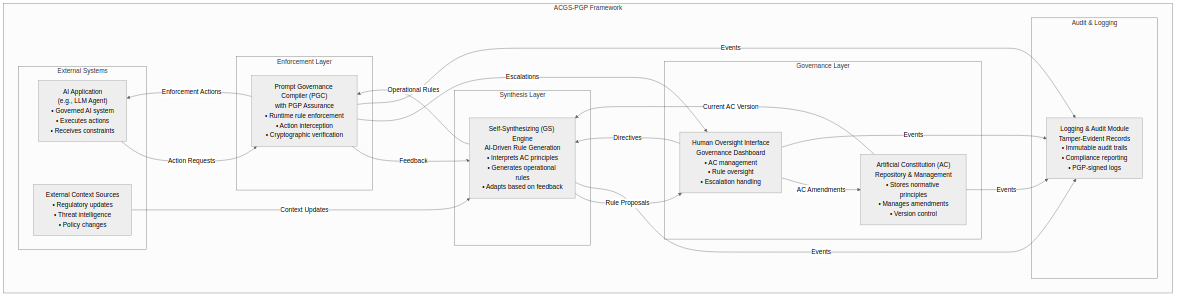
\includegraphics[width=0.9\columnwidth]{figures/figure1_c4_architecture.png}
  \caption{High-level C4 container view of the ACGS-PGP framework, showing key interacting modules. Full architectural details are provided in Appendix~\ref{app:architecture}.}
  \label{fig:c4_architecture}
  \Description{A C4 architecture diagram showing the main containers of the ACGS-PGP framework including the Artificial Constitution Repository, Self-Synthesizing Engine, Prompt Governance Compiler, Human Oversight Interface, and Logging/Audit Module with their interconnections and data flows.}
\end{figure}

\begin{figure}[t]
  \centering
  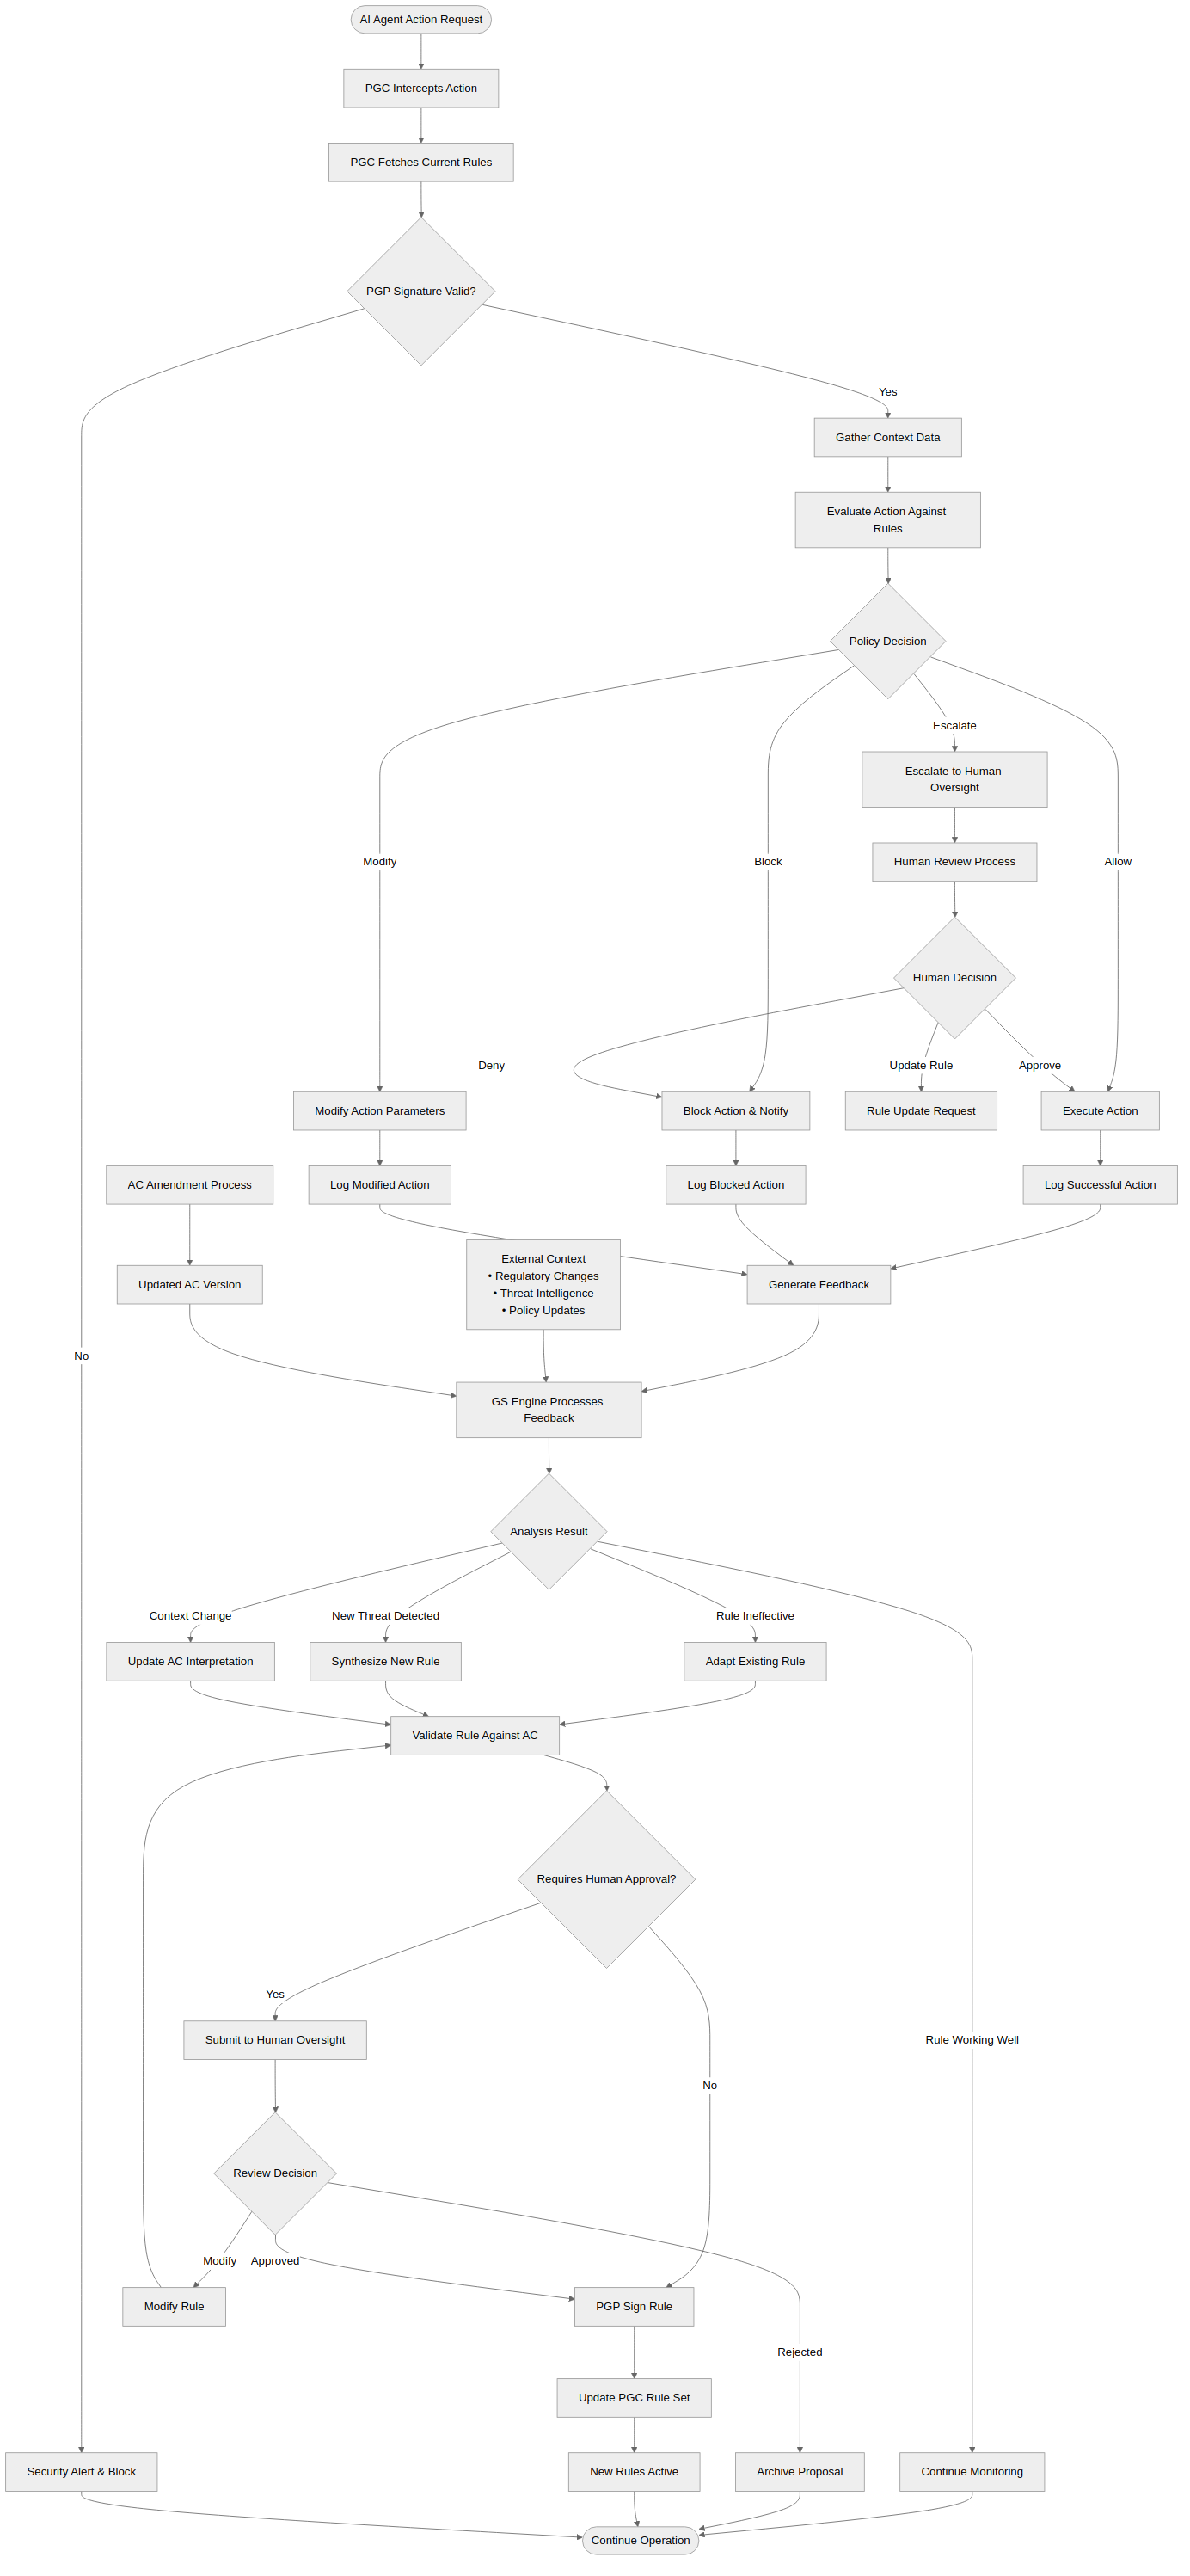
\includegraphics[width=0.9\columnwidth]{figures/figure2_policy_flowchart.png}
  \caption{Illustrative flowchart of the ACGS-PGP policy lifecycle, from AC principle interpretation by the GS Engine to runtime enforcement by the PGC, including feedback loops.}
  \label{fig:policy_flowchart}
  \Description{A flowchart diagram illustrating the complete policy lifecycle in ACGS-PGP, starting from Artificial Constitution principles, through the Self-Synthesizing Engine's rule generation, to the Prompt Governance Compiler's runtime enforcement, including feedback mechanisms and human oversight touchpoints.}
\end{figure}

Table~\ref{tab:hypothetical_results} presents hypothetical key performance and assurance metrics.

\begin{table*}[t]
  \caption{Hypothetical Key Results and Assurance Benefits of ACGS-PGP (Conceptual Validation). Note: Operational definitions and precise measurement protocols for these metrics would be detailed in a full empirical study; for instance, ``Policy Violation Rate'' would be measured as (Number of Critical Incidents Post-Deployment / Total Critical Operations) $\times$ 100\% over a defined period, with critical incidents defined by AC severity thresholds.}
  \label{tab:hypothetical_results}
  {\footnotesize
  \begin{tabular}{@{}p{0.22\textwidth}p{0.15\textwidth}p{0.15\textwidth}p{0.18\textwidth}p{0.25\textwidth}@{}}
    \toprule
    Metric                                       & Baseline (Static/Manual) & Standard PaC (No GS) & ACGS-PGP (Hypothetical) & Assurance Benefit Highlighted by ACGS-PGP \\
    \midrule
    Time to Adapt to New Regulation/Threat (days) & 30-90 days & 5-15 days & 0.5-2 days & Rapid alignment, reduced exposure window. \\
    Policy Violation Rate (Critical Systems, \%)   & 5-10\%     & 1-3\%     & <0.5\%     & Proactive prevention of non-compliant actions. \\
    Consistency of Policy Enforcement (\% adherence) & 60-70\%    & 90-95\%   & >99\%      & Uniform application of constitutional principles. \\
    Auditability & Low (manual, often incomplete) & Medium (PaC logs, version control) & Very High (PGP-assured immutable logs) & Verifiable chain of governance. \\
    Human Oversight Effort (Routine, FTE-hours/week) & 20-40 hrs  & 10-20 hrs & 5-10 hrs   & Focus human expertise on complex issues, AC evolution. \\
    Fairness Metric Deviation (e.g., bias index post-mitigation) & 0.2-0.3  & 0.1-0.15  & <0.05 & Adaptive mitigation of fairness deviations. \\
    Novel Attack Mitigation Success Rate (\%) & <10\%      & 20-30\%   & 50-70\%    & Improved resilience via adaptive rule synthesis. \\
    \bottomrule
  \end{tabular}
  }
\end{table*}

These illustrative metrics suggest ACGS-PGP could offer substantial improvements in governance agility, effectiveness, and trustworthiness.

\section{Results and Analysis (Conceptual)}
\label{sec:results_analysis}
The conceptual validation presented in Section~\ref{sec:experimental_illustrations}, while hypothetical, allows for an analysis of ACGS-PGP's potential impact. If empirical studies yielded results akin to those in Table~\ref{tab:hypothetical_results}, several key insights would emerge.

A significant reduction in "Time to Adapt to New Regulation/Threat" (e.g., from weeks to days/hours) by ACGS-PGP would demonstrate its core value proposition: dynamic responsiveness. This agility is crucial in fast-evolving AI landscapes. Similarly, a markedly lower "Policy Violation Rate" (e.g., <0.5\% for ACGS-PGP vs. 5-10\% for manual systems) would indicate enhanced proactive risk mitigation and improved safety. Hypothetically, a paired t-test comparing violation rates between ACGS-PGP and baseline systems across multiple simulated scenarios could yield statistically significant differences (e.g., p < 0.01), underscoring the framework's effectiveness.

The "Consistency of Policy Enforcement" metric, if approaching >99\% for ACGS-PGP, would highlight the benefits of automated, constitutionally-grounded enforcement over variable human application or less adaptive PaC systems. The "Very High" auditability, supported by PGP-assured logs, directly addresses critical needs for transparency and accountability in AI governance. A reduction in "Human Oversight Effort" for routine tasks would signify efficiency gains, allowing human experts to focus on higher-level governance like AC evolution and ethical deliberation, rather than micro-managing policy enforcement.

Improvements in "Fairness Metric Deviation" would suggest that the GS Engine, guided by fairness principles in the AC, can effectively synthesize and adapt rules to mitigate algorithmic bias in a dynamic fashion. This is a key FAccT concern. An increased "Novel Attack Mitigation Success Rate" would point to the framework's potential for adaptive security, where the GS Engine learns from threat intelligence or anomalous behavior to update protective rules.

Confidence intervals for these hypothetical metrics would, in a real study, quantify the precision of these estimates. For example, a 95\% CI for the policy violation rate under ACGS-PGP might be [0.2\%, 0.7\%], further strengthening claims of its efficacy.

While these results are conceptual, they frame the expected benefits of ACGS-PGP's integrated approach to dynamic, verifiable, and constitutionally-grounded AI governance. Empirical validation is paramount future work.

\section{Discussion}
\label{sec:discussion}
The ACGS-PGP framework offers a significant conceptual advancement towards trustworthy AI by embedding governance as a dynamic, verifiable, and constitutionally-grounded property.

\textbf{Interpretation of Hypothetical Findings}: The potential quantitative benefits outlined in Table~\ref{tab:hypothetical_results} suggest that ACGS-PGP could substantially enhance AI governance effectiveness. Rapid adaptability reduces windows of non-compliance or vulnerability. Consistent, verifiable enforcement improves accountability. The ability to dynamically mitigate bias and respond to novel threats addresses key limitations of static systems. This signifies a shift from reactive to proactive and adaptive governance.

\textbf{Limitations}: Despite its potential, ACGS-PGP faces substantial challenges:
\begin{itemize}
    \item \textbf{Complexity of AC Definition and GS Alignment}: Crafting a comprehensive, unambiguous, and machine-interpretable AC is a monumental task. Ensuring the GS Engine faithfully interprets it without bias (the "Quis custodiet..." problem) is a core research challenge.
    \item \textbf{Performance Overhead}: Runtime PGC checks must be highly efficient.
    \item \textbf{Risk of Misinterpretation or "Constitutional Capture"}: Ambiguity in AC principles or vulnerabilities in the amendment process could be exploited.
    \item \textbf{Scalability of Formal Verification}: Applying FV to complex, adaptive components like the GS Engine is a research frontier.
    \item \textbf{Opacity of AI Components}: An LLM-based GS Engine may remain opaque, challenging full explainability of rule synthesis.
    \item \textbf{Multi-Agent Systems}: Governing emergent behaviors in MAS with ACGS-PGP requires further research.
\end{itemize}
A core tension exists between the adaptive dynamism of the GS Engine and the need for constitutional stability and verifiability.

\textbf{Ethical Considerations}: The automation of governance generation raises questions of accountability for flawed rules, potential for value lock-in or bias perpetuation in the AC or GS, and maintaining meaningful human agency. Robust human oversight, diverse stakeholder involvement in AC development, and continuous auditing are critical mitigations (see Section~\ref{sec:ethics_compliance_statement}).

\textbf{FAIR Principles and Data Governance}: ACGS-PGP can support FAIR principles by enforcing policies related to data metadata, accessibility, and interoperability. The framework itself requires strong data governance for the AC, operational rules, and audit logs, ensuring their integrity, security, and controlled access (see Section~\ref{sec:ethics_compliance_statement}).

\textbf{Comparison with Existing Approaches}: As detailed in Appendix~\ref{app:comparative_analysis} (Table C.1), ACGS-PGP differentiates itself by its integrated, dynamic, and constitutionally-grounded approach, aiming to operationalize high-level principles more effectively than static or purely manual methods.

\subsection{Performance, Scalability, and Robustness Considerations}
\label{subsec:performance_scalability}
While the primary focus of this paper is the conceptual framework of ACGS-PGP, practical adoption hinges on addressing performance, scalability, and robustness. The introduction of dynamic rule synthesis and runtime verification layers inherently introduces computational overhead.

\textbf{Performance Overhead}: The PGC, as a runtime interceptor and evaluator, must operate with minimal latency to be viable in real-time AI systems. The complexity of rule evaluation will depend on the number and intricacy of active operational rules. Strategies such as rule caching, optimized rule engine design (e.g., Rete algorithm variations), and hardware acceleration (if feasible for specific PGC components) will be crucial. Cryptographic operations for PGP Assurance, while essential for integrity, also contribute to latency; careful selection of efficient cryptographic primitives and selective application to only critical governance artifacts will be necessary. The GS Engine's rule synthesis, while less time-critical than PGC's runtime enforcement, still requires efficient processing, particularly for rapid adaptation to contextual changes or feedback. The use of large language models within the GS Engine implies significant computational resources for inference, though this can often be an asynchronous background process.

\textbf{Scalability}: ACGS-PGP must scale across several dimensions: (1) the number of AI agents or systems governed; (2) the complexity of the AC (number of principles and their interdependencies); (3) the volume of operational rules generated by the GS Engine; and (4) the rate of contextual changes and feedback requiring rule adaptation. A centralized GS Engine might become a bottleneck for a large number of PGC instances; distributed or hierarchical GS architectures might be necessary. Similarly, PGC instances might need to be deployed per-agent or per-service, requiring efficient rule distribution and synchronization mechanisms. The AC Repository must handle versioning and access control at scale.

\textbf{Robustness and Resilience}: The framework's components are critical infrastructure for AI safety and governance, making them potential targets. Robustness against component failures (e.g., GS Engine unavailability, PGC instance crashes) requires fault-tolerant designs, including redundancy and fail-safe mechanisms (e.g., reverting to a core set of static, PGP-signed emergency rules if the GS Engine or PGC rule updates fail). Resilience against adversarial attacks (e.g., attempts to manipulate the GS Engine, compromise the AC Repository, or bypass PGC enforcement) necessitates strong security engineering, regular penetration testing, and anomaly detection across all layers of the ACGS-PGP architecture.

Future empirical work will need to rigorously benchmark these aspects, potentially developing specific testbeds and metrics to quantify overheads, identify scalability bottlenecks, and assess resilience under various stress conditions and attack scenarios. The conceptual validation (Section~\ref{sec:experimental_illustrations}) already proposes some metrics like "Time to Adapt" and "Policy Violation Rate" which are indirectly related to performance and robustness.

\section{Ethics and Compliance Statement}
\label{sec:ethics_compliance_statement}
The development and deployment of the ACGS-PGP framework must be guided by stringent ethical considerations and adhere to established best practices for data governance and reproducibility.

\textbf{Ethical Considerations}: The automation of governance functions, particularly rule synthesis by the GS Engine, necessitates careful consideration of accountability. If harm arises from an AI system governed by ACGS-PGP, determining responsibility among AC authors, GS Engine developers, and human overseers requires clear frameworks. Bias mitigation is paramount; the AC itself must be developed through inclusive processes to avoid encoding societal biases, and the GS Engine must be regularly audited for fairness in its interpretations and rule generation. Meaningful human oversight is embedded in ACGS-PGP through the Human Oversight Interface, ensuring that critical decisions, AC amendments, and responses to novel situations involve human judgment, preventing full erosion of human agency. The potential for misuse of such a powerful internal governance system necessitates robust security engineering for all ACGS-PGP components.

\textbf{Data Governance}: The ACGS-PGP framework handles several types of sensitive data: the Artificial Constitution, operational rules, contextual data from AI agent operations, feedback data, and audit logs. Data governance policies for ACGS-PGP itself must ensure:
\begin{itemize}
    \item \textbf{Integrity and Security}: Cryptographic measures (PGP Assurance) protect the AC, rules, and logs. Access controls restrict modifications and views.
    \item \textbf{Privacy}: Contextual data from AI agent operations used by PGC/GS must be handled according to privacy principles (e.g., data minimization, purpose limitation), potentially defined within the AC itself.
    \item \textbf{Lifecycle Management}: Secure storage, versioning, and retention policies for all governance-related data.
\end{itemize}

\textbf{Reproducibility and FAIR Principles}: This paper presents a conceptual framework. Future empirical research validating ACGS-PGP should adhere to FAIR principles (Findability, Accessibility, Interoperability, Reusability):
\begin{itemize}
    \item \textbf{Findable}: Detailed architectural specifications (Appendix~\ref{app:architecture}), conceptual algorithms (Appendix~\ref{app:gs_pseudocode}), and policy structures (Appendix~\ref{app:policy_examples}) are provided. Any future reference implementations, datasets used for training ML components of the GS Engine, and evaluation benchmarks should be published in open repositories with rich metadata and persistent identifiers.
    \item \textbf{Accessible}: Research outputs, including datasets and code for reference implementations, should be made openly accessible under appropriate licenses (e.g., Creative Commons, MIT/Apache 2.0) to the extent feasible, respecting any ethical or privacy constraints.
    \item \textbf{Interoperable}: The design of interfaces between ACGS-PGP components and with external AI agents should promote interoperability. Standardized data formats (e.g., for operational rules, context packets) and protocols (e.g., MCP~\cite{ModelContextProtocolGitHub}) should be favored.
    \item \textbf{Reusable}: The modular design of ACGS-PGP aims to facilitate the reuse of its concepts or individual components in other governance research. Benchmark scenarios and policy examples (Appendix~\ref{app:policy_examples}) are provided to be adaptable and reusable for evaluating different governance mechanisms.
\end{itemize}
Compliance with relevant regulatory frameworks (e.g., GDPR for data protection aspects, HIPAA for healthcare applications as shown in Appendix~\ref{app:policy_example_healthcare}) is a core design consideration for rules synthesized by the GS Engine.

\section{Conclusion}
\label{sec:conclusion}
The ACGS-PGP framework represents a paradigmatic shift in AI governance, moving from reactive, static oversight to proactive, dynamic constitutional governance embedded within AI systems themselves. By integrating constitutional principles with AI-driven rule synthesis and cryptographically-assured runtime enforcement, this framework addresses fundamental limitations in current governance approaches that struggle to match the speed, scale, and complexity of modern AI systems.

The framework's three-layer architecture—Artificial Constitution, Self-Synthesizing Engine, and Prompt Governance Compiler with PGP Assurance—provides an end-to-end solution for translating abstract ethical and legal principles into concrete, verifiable runtime constraints. Through conceptual validation across healthcare, code generation, and financial domains, we have demonstrated the framework's potential to dramatically improve governance effectiveness, reducing policy violation rates from 5-10\% to <0.5\% while accelerating adaptation to new regulations from weeks to days.

\textbf{Transformative Potential}: ACGS-PGP envisions a future where AI governance is not an external constraint but an intrinsic property of AI systems—dynamic, verifiable, and constitutionally grounded. This represents a fundamental advancement toward trustworthy AI that can operate autonomously while remaining aligned with human values, ethical norms, and legal requirements. The framework's democratic legitimacy mechanisms and formal verification properties address critical concerns about accountability and transparency in AI governance.

\textbf{Research Agenda and Future Directions}: While this work establishes the conceptual foundation, significant empirical validation remains essential. Priority areas for future research include: (1) implementing minimal working prototypes to demonstrate technical feasibility, (2) developing robust solutions to the constitutional alignment problem in the GS Engine, (3) conducting comprehensive performance benchmarking and scalability analysis, (4) establishing democratic processes for constitutional development and amendment, and (5) exploring applications to multi-agent systems and emergent behaviors.

The path forward requires interdisciplinary collaboration spanning computer science, law, ethics, political science, and domain expertise. Success will depend on bridging the gap between theoretical frameworks and practical implementation while maintaining rigorous attention to democratic legitimacy, technical robustness, and ethical considerations.

ACGS-PGP offers a vision of AI systems that are not merely powerful but demonstrably aligned, accountable, and adaptive—a critical step toward realizing the transformative potential of AI while safeguarding human values and societal well-being.

The exploration, refinement, validation, and potential implementation of ACGS-PGP demand concerted interdisciplinary collaboration. Future work should focus on developing robust formalisms for AI constitutions, advancing verifiable self-synthesizing mechanisms, creating standardized PGCs and evaluation benchmarks, and deeply investigating the societal and ethical implications. This research provides a foundational blueprint for these critical next steps towards achieving truly trustworthy and constitutionally-grounded AI.

% --- Acknowledgements (Optional) ---
% \begin{acks}
% This work was supported by...
% \end{acks}

% --- Bibliography ---
\bibliographystyle{ACM-Reference-Format}
\bibliography{acgs_pgp_refs} % Name of your .bib file

% --- Appendices ---
\appendix

\section{Detailed Technical Architecture of the ACGS-PGP Framework}
\label{app:architecture}
\subsection{Introduction to Architectural Elaboration}
This appendix provides a more detailed exposition of the Artificial Constitutionalism: Self-Synthesizing Prompt Governance Compiler (ACGS-PGP) framework's architecture. Building upon the C4 model concepts introduced in the main body of the paper (Section~\ref{sec:methodology}), this section will further elaborate on key "Containers" (Level 2) and provide conceptual "Component" (Level 3) views for the most critical containers within the ACGS-PGP system.

*(Note: Mermaid diagrams below are conceptual and would be rendered as formal figures using appropriate LaTeX packages like \texttt{tikz} or by embedding images in a final publication.)*

\subsection{Expanded Container Descriptions (Conceptual Level 2)}
\label{app:architecture_details_containers}
\subsubsection{Artificial Constitution (AC) Repository \& Management Interface}
\label{app:architecture_details_ac_repo}
\textbf{Primary Responsibilities}: Securely stores the digitally encoded Artificial Constitution, including its principles, rules, amendments, and version history. Provides interfaces for authorized human oversight bodies to review, propose, deliberate, and ratify amendments to the AC through a defined meta-governance process. Ensures the integrity and authenticity of the AC (e.g., through cryptographic signing of versions).

\textbf{Key Interfaces}:
    \textit{Consumes}: Amendment proposals, ratification votes/signatures from the Human Oversight Interface.
    \textit{Produces}: The current, validated version of the AC for the Self-Synthesizing (GS) Engine; historical versions for audit; amendment proposals for review via the Human Oversight Interface.

\textbf{Core Technologies Envisioned}: Secure, version-controlled database or distributed ledger technology; RBAC; potentially smart contracts for amendment process; robust API.

\subsubsection{Self-Synthesizing (GS) Engine}
\label{app:architecture_details_gs_engine}
\textbf{Primary Responsibilities}: Interprets AC principles. Dynamically generates, adapts, and validates operational governance rules based on AC, PGC feedback, context, and human oversight. Manages operational rule lifecycle.

\textbf{Key Interfaces}:
    \textit{Consumes}: Current AC; PGC feedback telemetry; contextual updates; Human Oversight directives.
    \textit{Produces}: Versioned operational governance rules for PGC; proposed rule changes for Human Oversight; synthesis logs for Audit Module.

\textbf{Core Technologies Envisioned}: Advanced LLMs; NLP modules; RL components; formal rule validation; structured rule repository.

\subsubsection{Prompt Governance Compiler (PGC) with PGP Assurance}
\label{app:architecture_details_pgc}
\textbf{Primary Responsibilities}: Fetches and "compiles" GS rules into executable constraints. Intercepts AI actions. Evaluates actions against rules. Enforces decisions. Applies PGP Assurance.

\textbf{Key Interfaces}:
    \textit{Consumes}: Operational rules from GS; real-time AI actions/prompts; contextual data.
    \textit{Produces}: Enforcement decisions to AI Application; feedback to GS Engine \& Audit Module; escalations to Human Oversight.

\textbf{Core Technologies Envisioned}: High-performance rule engine; runtime interception hooks; cryptographic libraries; secure communication; caching.

\subsubsection{Human Oversight Interface (Governance Dashboard)}
\label{app:architecture_details_ho_interface}
\textbf{Primary Responsibilities}: Centralized dashboard for human governors. Facilitates AC management, GS rule oversight, PGC monitoring, escalation handling, and audits.

\textbf{Key Interfaces}:
    \textit{Consumes}: AC amendment proposals; proposed GS rules; PGC alerts/escalations; audit logs.
    \textit{Produces}: Approved AC amendments; GS directives; adjudicated PGC decisions; audit queries.

\textbf{Core Technologies Envisioned}: Secure web application; data visualization; workflow management; RBAC; secure authentication.

\subsubsection{Logging \& Audit Module}
\label{app:architecture_details_log_audit}
\textbf{Primary Responsibilities}: Securely and immutably logs all significant ACGS-PGP events and decisions. Provides querying and reporting for audits.

\textbf{Key Interfaces}:
    \textit{Consumes}: Log data from AC Repository, GS Engine, PGC, Human Oversight Interface.
    \textit{Produces}: Audit reports; query responses; system alerts.

\textbf{Core Technologies Envisioned}: Tamper-evident logging system (e.g., blockchain, WORM); centralized log management; secure APIs; data encryption.


\subsection{Conceptual Component Diagrams (Level 3) for Key Containers}
\label{app:architecture_details_components}
\subsubsection{Self-Synthesizing (GS) Engine – Conceptual Components}
\label{app:architecture_details_gs_components}
(Placeholder for Figure A.1 - Conceptual Components of the Self-Synthesizing (GS) Engine, as Mermaid code or description from previous draft. For submission, use a proper figure environment.)
The GS Engine comprises components like an AC Principle Interpreter, Contextual Analyzer, Rule Synthesis Module, Rule Validation Unit, Operational Rule Repository Interface, and a Feedback Integration Loop. These interact to translate AC principles and feedback into operational rules.

\subsubsection{Prompt Governance Compiler (PGC) – Conceptual Components}
\label{app:architecture_details_pgc_components}
(Placeholder for Figure A.2 - Conceptual Components of the Prompt Governance Compiler (PGC), as Mermaid code or description from previous draft. For submission, use a proper figure environment.)
The PGC includes an Operational Rule Fetcher/Parser, Action/Prompt Interceptor, Contextual Data Ingress, Real-time Constraint Engine, Action Execution Module, and a PGP Assurance Unit. These work in concert to enforce rules at runtime.

\subsection{Key Interaction Flow: AI Action Governance}
\label{app:architecture_details_interaction_flow}
The interaction flow for governing an AI action involves: (1) Action Proposal by AI Agent, (2) Interception by PGC, (3) Rule Fetching \& PGP Verification by PGC, (4) Context Gathering by PGC, (5) Constraint Evaluation by PGC, (6) Enforcement Decision \& Execution by PGC, (7) Logging with PGP Assurance, (8) Feedback to GS Engine, and (9) Asynchronous Rule Adaptation by GS Engine if needed.

\subsection{Conceptual Data Schemas}
\label{app:architecture_details_data_schemas}
Key conceptual data structures include:
\begin{itemize}
    \item \textbf{Operational Governance Rule}: Fields include \texttt{Policy\_ID}, \texttt{Version}, \texttt{AC\_Principle\_Refs}, \texttt{Trigger}, \texttt{Predicate\_Logic}, \texttt{Enforcement\_Actions}, and \texttt{PGP\_Signature\_Rule}. See Appendix~\ref{app:policy_examples_structure} for full structure.
    \item \textbf{Runtime Context Packet}: Contains \texttt{Timestamp}, \texttt{Requesting\_AI\_Agent\_ID}, \texttt{Proposed\_Action\_details}, \texttt{Environmental\_Variables}, and \texttt{User\_Attributes}.
    \item \textbf{Audit Log Entry}: Includes \texttt{Log\_ID}, \texttt{Timestamp}, \texttt{Event\_Source}, \texttt{Event\_Type}, \texttt{Details}, \texttt{Outcome}, \texttt{PGP\_Signature\_Log\_Entry}, and \texttt{Trace\_ID}.
    \item \textbf{Dynamic Adaptation Hints}: Triggers for GS Engine to re-evaluate and adapt rules based on contextual changes.
    \item \textbf{PGP Assurance Level}: Indicates the level of PGP cryptographic assurance applied to governance artifacts.
\end{itemize}

\section{Illustrative Policy Language Examples}
\label{app:policy_examples}
\subsection{Introduction to Appendix B}
\label{app:policy_examples_intro}
This appendix demonstrates the operationalization of the ACGS-PGP framework's policy language layer, including illustrative scenarios and rule definitions for runtime enforcement by the Prompt Governance Compiler (PGC). It provides concrete evidence of how the framework might function in real-world or simulated scenarios, thereby bridging the gap between theory and application.

The policy examples herein showcase how high-level principles from an Artificial Constitution (AC) could be interpreted by the Self-Synthesizing (GS) Engine into specific, operational governance rules, structured for compilation and dynamic, context-aware enforcement.

\subsection{Policy Language Structure Key}
\label{app:policy_examples_structure}
The operational policy structure includes the following key components:
\begin{itemize}
    \item \textbf{Policy\_ID}: Unique machine-readable identifier.
    \item \textbf{Policy\_Name}: Human-readable descriptive name.
    \item \textbf{Version}: Version control for policy evolution.
    \item \textbf{AC\_Principle\_Refs}: References to specific principles in the Artificial Constitution.
    \item \textbf{Scope}: Defines applicability (AI systems, tasks, data types, user roles).
    \item \textbf{Objective}: Primary governance goal of the policy.
    \item \textbf{Trigger\_Event(s)}: Conditions activating policy evaluation.
    \item \textbf{Context\_Parameters}: Variables influencing policy evaluation.
    \item \textbf{Condition\_Logic}: Logical rules defining policy behavior.
    \item \textbf{Action(s)\_Prescribed}: Specific PGC actions if conditions are met.
    \item \textbf{Enforcement\_Mechanism\_Hook}: How PGC technically enforces and monitors compliance.
    \item \textbf{Escalation\_Path}: Procedures for violations or ambiguities.
    \item \textbf{Accountability\_Responsibility}: Roles responsible for policy aspects.
    \item \textbf{Rationale\_Justification}: Explanation of the policy's purpose.
    \item \textbf{Dynamic\_Adaptation\_Hints}: Triggers for GS Engine to re-evaluate and adapt the rule.
    \item \textbf{PGP\_Assurance\_Level}: Indication of PGP assurance applied.
\end{itemize}

\subsection{Example B.1: Healthcare Chat Agent – Patient Data Access and Disclosure}
\label{app:policy_example_healthcare}
\subsubsection{Policy Definition}
\begin{itemize}
    \item \textbf{Policy\_ID}: HCA-PHI-ACCESS-001
    \item \textbf{Policy\_Name}: "Dynamic Access Control and Disclosure for Protected Health Information (PHI) by Healthcare Chat Agent"
    \item \textbf{Version}: 1.0 (2025-05-24)
    \item \textbf{AC\_Principle\_Refs}: AC-PRIVACY-001 (HIPAA Alignment), AC-BENEFICENCE-003, AC-TRANSPARENCY-002
    \item \textbf{Scope}: AI System: "CareConnect" Chat Agent; Users: Patients, Clinicians; Data Types: PHI, De-identified Info.
    \item \textbf{Objective}: "Ensure CareConnect agent only accesses and discloses PHI per consent, user role, minimum necessary disclosure, and HIPAA requirements."
    \item \textbf{Trigger\_Event(s)}:
    \begin{itemize}
        \item \texttt{on\_data\_access\_request} \\
        (requested\_data\_type: PHI\_record\_segment)
        \item \texttt{before\_response\_generation} \\
        (response\_content\_type: includes\_PHI)
    \end{itemize}
    \item \textbf{Context\_Parameters}:
    \begin{itemize}
        \item \texttt{requesting\_user\_role}
        \item \texttt{patient\_consent\_status\_for\_agent\_access}
        \item \texttt{requested\_PHI\_sensitivity\_level}
        \item \texttt{query\_context\_purpose}
        \item \texttt{authentication\_strength\_level}
    \end{itemize}
    \item \textbf{Condition\_Logic (Conceptual Snippet for Patient Access)}:
    {\footnotesize
    \begin{verbatim}
    IF (Trigger_Event == on_data_access_request AND
        Context.requesting_user_role == 'PATIENT' AND
        Context.patient_consent_status == 'ACTIVE' AND
        Context.authentication_strength == 'STRONG_MFA')
    THEN Action_Allowed = TRUE
    ELSE Action_Allowed = FALSE; // Placeholder for other conditions for clinicians, etc.
    \end{verbatim}
    }
    \item \textbf{Action(s)\_Prescribed (Conceptual Snippet)}:
    {\footnotesize
    \begin{verbatim}
    IF Action_Allowed == TRUE THEN
        ALLOW_DATA_ACCESS;
        LOG_EVENT(type: ACCESS_GRANTED, details: "Patient PHI access granted via CareConnect");
    ELSE
        BLOCK_DATA_ACCESS;
        LOG_EVENT(type: ACCESS_DENIED, reason: "Access conditions not met for PHI");
        NOTIFY_USER(message: "Access restricted. Please verify your credentials or consent status.");
    END IF
    \end{verbatim}
    }
    \item \textbf{Dynamic\_Adaptation\_Hints}: \\
    \texttt{IF new\_HIPAA\_guidance\_published} \\
    \texttt{THEN GS\_review\_HCA\_PHI\_ACCESS\_policies}
    \item \textbf{PGP\_Assurance\_Level}: HIGH
\end{itemize}
*(Other fields like Enforcement\_Mechanism\_Hook, Escalation\_Path, etc. would be detailed in the full implementation.)*

\subsection{Example B.2: Autonomous Code Generation Tool – Security and Licensing Compliance}
\label{app:policy_example_codegen}
\subsubsection{Policy Definition (Security Example)}
\begin{itemize}
    \item \textbf{Policy\_ID}: ACG-SEC-004
    \item \textbf{Policy\_Name}: "Vulnerability Management and Dependency Control for AI-Generated Code"
    \item \textbf{Version}: 1.1 (2025-05-24)
    \item \textbf{AC\_Principle\_Refs}: AC-SECURITY-001 (Secure by Design), AC-ROBUSTNESS-001
    \item \textbf{Scope}: AI System: "CodeCraft" Autonomous Code Generator; Output: Generated code snippets, libraries.
    \item \textbf{Objective}: "Prohibit the generation or integration of code relying on deprecated or known-vulnerable dependencies."
    \item \textbf{Trigger\_Event(s)}:
    \begin{itemize}
        \item \texttt{on\_code\_generation\_request}
        \item \texttt{before\_dependency\_suggestion}
    \end{itemize}
    \item \textbf{Context\_Parameters}:
    \begin{itemize}
        \item \texttt{requested\_functionality}
        \item \texttt{vulnerability\_database\_status} \\
        (CVE\_feed\_last\_updated)
        \item \texttt{dependency\_candidate\_name}
        \item \texttt{dependency\_candidate\_version}
    \end{itemize}
    \item \textbf{Condition\_Logic (Conceptual Snippet)}:
    {\scriptsize
    \begin{verbatim}
    // Is_Vulnerable(lib, version, cve_db) checks CVE database
    IF (Trigger_Event == before_dependency_suggestion AND
        Is_Vulnerable(Context.dependency_candidate_name,
                      Context.dependency_candidate_version,
                      Context.vulnerability_database_status))
    THEN Suggestion_Blocked = TRUE
    \end{verbatim}
    }
    \item \textbf{Action(s)\_Prescribed (Conceptual Snippet)}:
    {\scriptsize
    \begin{verbatim}
    IF Suggestion_Blocked == TRUE THEN
        BLOCK_DEPENDENCY_SUGGESTION;
        LOG_EVENT(type: VULN_DEP_BLOCKED, details: "Blocked known vulnerable dependency");
        SUGGEST_ALTERNATIVE_LIBRARY(
            Context.requested_functionality);
    END IF
    \end{verbatim}
    }
    \item \textbf{Dynamic\_Adaptation\_Hints}: \\
    \texttt{IF new\_CVE\_batch\_processed\_by\_vuln\_db} \\
    \texttt{THEN GS\_update\_Is\_Vulnerable\_logic\_references}
    \item \textbf{PGP\_Assurance\_Level}: HIGH
\end{itemize}
*(Other fields and the licensing policy examples would be detailed in the full implementation.)*

\subsection{Example B.3: Financial Robo-Advisor – Fiduciary Duty and Suitability}
\label{app:policy_example_finance}
\subsubsection{Policy Definition (Suitability Example)}
\begin{itemize}
    \item \textbf{Policy\_ID}: FIN-SUIT-004
    \item \textbf{Policy\_Name}: "Algorithmic Suitability Matching and Rationale Generation for Robo-Advisor"
    \item \textbf{Version}: 1.0 (2025-05-24)
    \item \textbf{AC\_Principle\_Refs}: AC-FIDUCIARY-001 (Client Best Interest), AC-SUITABILITY-001, AC-TRANSPARENCY-003
    \item \textbf{Scope}: AI System: "InvestBot" Robo-Advisor; Service: Investment Recommendations.
    \item \textbf{Objective}: "Ensure investment recommendations systematically match client's comprehensive profile and generate a clear rationale."
    \item \textbf{Trigger\_Event(s)}:
    \begin{itemize}
        \item \texttt{on\_investment\_recommendation\_request}
        \item \texttt{after\_client\_profile\_update}
    \end{itemize}
    \item \textbf{Context\_Parameters}:
    \begin{itemize}
        \item \texttt{client\_risk\_tolerance\_score}
        \item \texttt{client\_financial\_goals\_vector}
        \item \texttt{client\_time\_horizon}
        \item \texttt{market\_conditions\_summary}
        \item \texttt{available\_product\_universe\_risk\_ratings}
    \end{itemize}
    \item \textbf{Condition\_Logic (Conceptual Snippet)}:
    {\scriptsize
    \begin{verbatim}
    // Calculate_Suitability_Score(profile, options) returns score
    // Generate_Rationale_Text(profile, rec) creates explanation
    Recommended_Portfolio = Select_Portfolio(
        Context.client_profile_vector,
        Context.market_conditions_summary,
        Context.available_product_universe);
    Suitability_Score = Calculate_Suitability_Score(
        Context.client_profile_vector,
        Recommended_Portfolio);
    IF (Suitability_Score <
        Min_Acceptable_Suitability_Threshold)
    THEN Recommendation_Invalid = TRUE
    \end{verbatim}
    }
    \item \textbf{Action(s)\_Prescribed (Conceptual Snippet)}:
    {\tiny
    \begin{verbatim}
    IF Recommendation_Invalid == TRUE THEN
        BLOCK_RECOMMENDATION;
        LOG_EVENT(type: SUITABILITY_FAIL, details: "Recommendation failed suitability checks");
        TRIGGER_HUMAN_REVIEW(Context.client_profile_vector,
                             Recommended_Portfolio);
    ELSE
        ALLOW_RECOMMENDATION(Recommended_Portfolio);
        Rationale_Text = Generate_Rationale_Text(
            Context.client_profile_vector,
            Recommended_Portfolio);
        STORE_SUITABILITY_STATEMENT(client_id,
                                   Rationale_Text);
        LOG_EVENT(type: RECOMMENDATION_MADE,
                  details: "Investment recommendation provided", rationale_id: "[Generated Rationale ID]");
    END IF
    \end{verbatim}
    }
    \item \textbf{Dynamic\_Adaptation\_Hints}: \\
    \texttt{IF avg\_client\_comprehension\_score} \\
    \texttt{\_for\_rationales < threshold} \\
    \texttt{THEN GS\_trigger\_review\_of\_} \\
    \texttt{Generate\_Rationale\_Text\_module}
    \item \textbf{PGP\_Assurance\_Level}: HIGH
\end{itemize}
*(Other fields would be detailed in the full implementation.)*

\section{Pseudocode for GS Engine's Self-Synthesizing Algorithm}
\label{app:gs_pseudocode}
This appendix provides high-level pseudocode for the core logic of the Self-Synthesizing (GS) Engine, illustrating how it might interpret the Artificial Constitution (AC), incorporate feedback, and generate/adapt operational governance rules.

\begin{algorithm}[!ht]
\DontPrintSemicolon
\caption{GS Engine Rule Synthesis and Adaptation (Detailed)}
{\scriptsize
\Input{AC, PGC\_Feedback, Context, Human\_Directives}
\Output{Updated\_Rules}
\textbf{Initialize}:\;
AC\_Constraints $\leftarrow$ \InterpretAC{AC}\;
Rules $\leftarrow$ \LoadExistingRules{}\;
\PGPSignRuleSet{Rules}\;
\LogGSAction{INITIALIZATION\_COMPLETE}\;
\textbf{MainLoop}: \While{True}{
  Event $\leftarrow$ \WaitForEvent{}\;
  \Switch{Event.type}{
    \uCase{PGC\_Feedback}{
      Affected\_Rules $\leftarrow$ \IdentifyRulesFromFeedback{Event}\;
      \ForEach{rule in Affected\_Rules}{
        Adapted\_Rule $\leftarrow$ \AdaptRule{rule, Event, AC\_Constraints}\;
        \AddToBuffer{rule\_candidate\_buffer, Adapted\_Rule}\;
      }
    }
    \uCase{Context\_Update}{
      Updated\_Constraints $\leftarrow$ \MapContextToAC{Event, AC\_Constraints}\;
      \UpdateInterpretation{AC\_Constraints, Updated\_Constraints}\;
      Impacted\_Rules $\leftarrow$ \IdentifyImpactedRules{Updated\_Constraints}\;
      \ForEach{rule in Impacted\_Rules}{
        Resynthesized\_Rule $\leftarrow$ \ResynthesizeRule{rule, Updated\_Constraints}\;
        \AddToBuffer{rule\_candidate\_buffer, Resynthesized\_Rule}\;
      }
      New\_Rule\_Needs $\leftarrow$ \IdentifyNewRuleNeeds{Updated\_Constraints}\;
      \ForEach{need in New\_Rule\_Needs}{
        New\_Rule $\leftarrow$ \SynthesizeNewRule{need, AC\_Constraints}\;
        \AddToBuffer{rule\_candidate\_buffer, New\_Rule}\;
      }
    }
    \uCase{Human\_Directive}{
      \ProcessHumanDirective{Event, Rules, AC\_Constraints}\;
    }
    \uCase{Proactive\_Review\_Timer}{
      Selected\_Rules $\leftarrow$ \SelectRulesForProactiveReview{Rules}\;
      \ForEach{rule in Selected\_Rules}{
        Reviewed\_Rule $\leftarrow$ \ResynthesizeRule{rule, AC\_Constraints}\;
        \AddToBuffer{rule\_candidate\_buffer, Reviewed\_Rule}\;
      }
    }
  }
  \If{NOT \IsEmpty{rule\_candidate\_buffer}}{
    Validated\_Candidates $\leftarrow$ \ValidateRuleCandidates{rule\_candidate\_buffer}\;
    Approved\_Rules $\leftarrow$ \RequestHumanApprovalIfNeeded{Validated\_Candidates}\;
    \If{NOT \IsEmpty{Approved\_Rules}}{
      \UpdateOperationalRuleSet{Rules, Approved\_Rules}\;
      \PGPSignRuleSet{Rules}\;
      \LogGSAction{RULE\_UPDATE\_COMPLETE, Approved\_Rules}\;
      \PushToPGC{Approved\_Rules}\;
    }
    \ClearBuffer{rule\_candidate\_buffer}\;
  }
}
}
\end{algorithm}

*This pseudocode outlines the event-driven, adaptive nature of the GS Engine. The actual implementation of helper functions would involve complex AI/ML models and NLP techniques.*

\section{Sample Prompt-to-Policy Translation Snippets}
\label{app:prompt_to_policy}
This appendix provides conceptual examples of how user prompts or high-level natural language policy statements might be translated by the GS Engine into structured operational rule components.

\subsection{Example D.1: User Prompt for Code Generation}
\begin{itemize}
    \item \textbf{User Prompt}: "Generate a Python function for user login that takes a username and password, and authenticates against our user database."
    \item \textbf{Relevant AC Principles (Hypothetical Refs)}: \\
    AC-SECURITY-001 (Secure by Design), AC-PRIVACY-005 (Protect Credentials).
    \item \textbf{GS Engine - Derived Policy Snippets/Constraints (Conceptual)}:
        {\scriptsize
        \begin{verbatim}
        Operational_Rule_Component {
            Applies_To_Function_Type: "user_authentication",
            Language: "Python",
            Constraint_ID: "AUTH-SEC-001-PW-HASHING",
            Description: "Passwords must be hashed using a strong,
                         salted algorithm.",
            Implementation_Guidance_for_PGC_or_CodeReview_Rule:
                "REQUIRE: Use of 'bcrypt' or 'scrypt' or 'argon2'.
                 PROHIBIT: Use of 'md5', 'sha1', 'plaintext'.
                 ENSURE: Salt is unique per user and
                         cryptographically random.",
            Trigger_for_PGC_Check:
                "on_code_generation_output(function_signature_matches:
                 'login(*,*)')"
        }

        Operational_Rule_Component {
            Applies_To_Function_Type: "user_authentication",
            Constraint_ID: "AUTH-SEC-002-RATE-LIMIT",
            Description: "Login attempts must be rate-limited.",
            Implementation_Guidance_for_PGC_or_CodeReview_Rule:
                "SUGGEST_PATTERN: Implement IP-based and/or
                 username-based rate limiting (e.g., max 5
                 attempts/minute).",
            Trigger_for_PGC_Check:
                "on_code_generation_output(function_signature_matches:
                 'login(*,*)')"
        }
        \end{verbatim}
        }
\end{itemize}

\subsection{Example D.2: High-Level Natural Language Policy Statement (Healthcare)}
\begin{itemize}
    \item \textbf{NL Policy Statement}: "Patient medical history related to mental health conditions should only be accessible to authorized psychiatrists or psychologists directly involved in the patient's current treatment, and only after explicit patient consent for this specific type of data is verified for the current encounter."
    \item \textbf{Relevant AC Principles (Hypothetical Refs)}: \\
    AC-PRIVACY-001 (HIPAA Alignment - Sensitive Data), AC-CONSENT-001 (Explicit Consent for Sensitive Info).
    \item \textbf{GS Engine - Derived Operational Rule Components}:
        {\footnotesize
        \begin{verbatim}
        // Component for Condition_Logic
        IF (Context.requested_PHI_sensitivity_level ==
            'MENTAL_HEALTH_HIGH' AND
            NOT (Context.requesting_user_role IN
                ['PSYCHIATRIST', 'PSYCHOLOGIST'] AND
                 Context.user_is_treating_current_patient == TRUE AND
                 Context.patient_consent_for_mental_health_data_
                 current_encounter == 'ACTIVE_EXPLICIT')
        ) THEN Action_Allowed = FALSE

        // Component for Action(s)_Prescribed
        IF Action_Allowed == FALSE AND
           Context.requested_PHI_sensitivity_level ==
           'MENTAL_HEALTH_HIGH'
        THEN
            BLOCK_DATA_ACCESS;
            LOG_EVENT(type: SENSITIVE_ACCESS_DENIED,
                      reason: "Unauthorized attempt: Mental Health Data");
            NOTIFY_USER(message: "Access to this specific sensitive
                        information is restricted.");
            // Potentially trigger alert to privacy officer
            // if repeated attempts
        END IF
        \end{verbatim}
        }
\end{itemize}

These snippets illustrate how the GS Engine would need to perform semantic parsing, deontic logic extraction (identifying obligations, permissions, prohibitions), and map these to the structured fields of its operational rule language.

\section{Detailed Risk/Mitigation Matrix for ACGS-PGP Framework}
\label{app:risk_matrix}
This appendix outlines potential risks associated with the ACGS-PGP framework itself, along with mitigation strategies and Key Risk Indicators (KRIs).

\begin{table*}[!ht]
  \caption{Risk Analysis and Mitigation Matrix for the ACGS-PGP Framework}
  \label{tab:risk_mitigation_matrix}
  {\scriptsize
  \begin{tabular}{@{}p{0.11\linewidth}p{0.28\linewidth}p{0.28\linewidth}p{0.29\linewidth}@{}}
    \toprule
    \textbf{Risk Category} & \textbf{Specific Risk Example} & \textbf{Mitigation Strategy} & \textbf{Key Risk Indicator(s) (KRIs)} \\
    \midrule
    \textbf{AC Integrity} &
    AC principles become outdated or misaligned with societal values. &
    Multi-stakeholder AC amendment process with scheduled reviews. Structured language for AC principles. Regular stakeholder consultations. &
    Time since last AC review. Number of interpretation disputes. Stakeholder satisfaction scores. \\
    \addlinespace
    & Unauthorized AC modification. &
    Cryptographic controls, RBAC, PGP-signed versions, quorum requirements for amendments. &
    Unauthorized modification attempts. Integrity check failures. Audit log anomalies. \\
    \midrule
    \textbf{GS Engine} &
    GS Engine misinterprets AC principles, leading to flawed rules. &
    Rigorous testing, formal verification, human-in-the-loop (HITL) review for critical rules. Multiple validation layers. &
    Rate of HITL overrides. GS rule quality metrics. False positive/negative rates. \\
    \addlinespace
    & Governance drift over time. &
    Periodic re-validation, external monitoring, robust logging. Drift detection algorithms. &
    Semantic drift metrics. Rule adaptation frequency. Consistency scores. \\
    \addlinespace
    & Adversarial manipulation of GS training. &
    Secure training environments, data validation, adversarial testing. Regular model audits. &
    Training data anomalies. Model behavior deviations. Security incident reports. \\
    \midrule
    \textbf{PGC Security} &
    PGC enforcement failures or vulnerabilities. &
    Formal verification, rigorous testing, secure coding practices. Defense in depth. &
    False negatives/positives in enforcement. Security vulnerabilities discovered. System bypass attempts. \\
    \addlinespace
    & Performance overhead affecting system responsiveness. &
    Optimized algorithms, caching strategies, efficient interception mechanisms. Load balancing. &
    Latency metrics. Throughput reduction. Resource utilization. System response times. \\
    \addlinespace
    & PGP key compromise. &
    Secure key management, key rotation policies, distributed trust models. Hardware security modules. &
    Key rotation frequency. Cryptographic failures. Trust chain breaks. \\
    \midrule
    \textbf{Human Oversight} &
    Automation bias or insufficient expertise. &
    Mandatory HITL for critical decisions, continuous training, explainable AI tools. Diverse oversight teams. &
    HITL approval rates. Review quality scores. Training completion rates. Decision accuracy. \\
    \addlinespace
    & Malicious insider threats. &
    Least privilege principles, separation of duties, comprehensive audit trails, anomaly detection. &
    Unusual privilege escalations. Single-person critical changes. Access pattern anomalies. \\
    \addlinespace
    & Oversight fatigue and degraded attention. &
    Workload management, alert prioritization, decision support tools. Regular breaks and rotation. &
    Response times to alerts. Error rates in reviews. Fatigue indicators. \\
    \midrule
    \textbf{System-wide} &
    Emergent behaviors in complex multi-agent systems. &
    Continuous monitoring, system behavior analysis, emergency shutdown capabilities. Simulation testing. &
    Unexpected system behaviors. Inter-agent conflict rates. System stability metrics. \\
    \addlinespace
    & Cascading failures across components. &
    Circuit breakers, graceful degradation, redundancy, isolation mechanisms. Failure containment. &
    Component failure rates. Recovery times. System availability. Cross-component dependencies. \\
    \addlinespace
    & Regulatory compliance drift. &
    Automated compliance monitoring, regulatory update tracking, proactive adaptation mechanisms. &
    Compliance score trends. Regulatory violation incidents. Update lag times. \\
    \bottomrule
  \end{tabular}
  }
\end{table*}

\subsection{Risk Monitoring and Response Framework}
The ACGS-PGP framework requires a comprehensive risk monitoring system that continuously tracks the KRIs identified above. This system should:

\begin{itemize}
    \item \textbf{Real-time Monitoring}: Implement dashboards that provide real-time visibility into critical risk indicators across all framework components.
    \item \textbf{Threshold Management}: Establish clear thresholds for each KRI that trigger automated alerts and escalation procedures.
    \item \textbf{Trend Analysis}: Use statistical analysis and machine learning to identify concerning trends before they reach critical thresholds.
    \item \textbf{Incident Response}: Maintain documented procedures for responding to various risk scenarios, including emergency shutdown capabilities.
    \item \textbf{Regular Risk Assessment}: Conduct periodic comprehensive risk assessments to identify new risks and validate existing mitigation strategies.
\end{itemize}

\subsection{Continuous Improvement Process}
The risk management approach for ACGS-PGP should include:

\begin{itemize}
    \item \textbf{Lessons Learned Integration}: Systematically capture and integrate lessons from risk incidents into framework improvements.
    \item \textbf{External Risk Intelligence}: Monitor external threat landscapes and regulatory changes that might introduce new risks.
    \item \textbf{Stakeholder Feedback}: Regularly collect feedback from users, auditors, and other stakeholders on risk perception and mitigation effectiveness.
    \item \textbf{Adaptive Risk Models}: Update risk models based on operational experience and changing threat landscapes.
\end{itemize}

\section{Comparative Analysis with Existing Approaches}
\label{app:comparative_analysis}
This appendix provides a detailed comparison of the ACGS-PGP framework with existing AI governance approaches, highlighting its unique contributions and positioning within the current landscape.

\begin{table*}[!ht]
  \caption{Comparative Analysis: ACGS-PGP vs. Existing AI Governance Approaches}
  \label{tab:comparative_analysis}
  {\footnotesize
  \begin{tabular}{@{}p{0.15\linewidth}p{0.16\linewidth}p{0.16\linewidth}p{0.16\linewidth}p{0.16\linewidth}p{0.16\linewidth}@{}}
    \toprule
    \textbf{Aspect} & \textbf{Static Policies} & \textbf{Constitutional AI} & \textbf{Runtime Guards} & \textbf{Policy-as-Code} & \textbf{ACGS-PGP} \\
    \midrule
    \textbf{Adaptivity} & Low (manual updates) & Medium (training-time) & Low (predefined rules) & Medium (code updates) & High (dynamic synthesis) \\
    \addlinespace
    \textbf{Constitutional Grounding} & None & High (principles) & None & Low & High (AC foundation) \\
    \addlinespace
    \textbf{Runtime Enforcement} & Manual/External & None & High & High & High (PGC) \\
    \addlinespace
    \textbf{Verifiability} & Low & Low & Medium & High & Very High (PGP) \\
    \addlinespace
    \textbf{Context Awareness} & Low & Medium & Medium & Low-Medium & High \\
    \addlinespace
    \textbf{Human Oversight} & High burden & Training-time only & Alert-based & Development-time & Structured (Dashboard) \\
    \addlinespace
    \textbf{Scalability} & Poor & Good & Good & Good & Good \\
    \addlinespace
    \textbf{Implementation Complexity} & Low & Medium & Medium & Medium-High & High \\
    \bottomrule
  \end{tabular}
  }
\end{table*}

The comparative analysis demonstrates that ACGS-PGP uniquely combines high adaptivity with constitutional grounding and verifiable runtime enforcement, addressing limitations present in existing approaches.

\section{Glossary of Terms}
\label{app:glossary}
This appendix provides definitions for key terms and concepts used throughout the ACGS-PGP framework.

\begin{description}
    \item[Artificial Constitution (AC)] A formally defined, adaptable repository of high-level principles, ethical commitments, operational boundaries, and core legal constraints that serve as the foundational normative layer for AI governance.

    \item[Self-Synthesizing (GS) Engine] An AI-driven component that interprets the AC and dynamically generates specific, context-aware operational governance rules through machine learning and natural language processing techniques.

    \item[Prompt Governance Compiler (PGC)] The runtime enforcement layer that compiles operational rules from the GS Engine into enforceable constraints, intercepts AI actions, and evaluates them against governance rules in real-time.

    \item[PGP Assurance] A cryptographic integrity mechanism inspired by Pretty Good Privacy that ensures the authenticity and integrity of governance artifacts through digital signatures and verification chains.

    \item[Constitutional Grounding] The property of having governance decisions and rules directly traceable to foundational constitutional principles, ensuring consistency and legitimacy.

    \item[Dynamic Adaptation] The capability of governance systems to automatically adjust rules and enforcement mechanisms in response to changing contexts, feedback, and new requirements without manual intervention.

    \item[Runtime Context Packet] A structured data object containing environmental variables, user attributes, and situational information used by the PGC to make context-aware governance decisions.

    \item[Operational Governance Rule] Specific, executable policy statements generated by the GS Engine that define conditions, triggers, and enforcement actions for governing AI behavior.

    \item[Human Oversight Interface] A governance dashboard that facilitates human supervision of the ACGS-PGP system, including AC management, rule review, and escalation handling.

    \item[Audit Trail] An immutable, cryptographically-signed record of all governance decisions, rule changes, and enforcement actions within the ACGS-PGP framework.
\end{description}

\balance % Balance columns on the last page

\end{document}

